%% LyX 2.3.7 created this file.  For more info, see http://www.lyx.org/.
%% Do not edit unless you really know what you are doing.
\documentclass[11pt,english,letterpaper, abstracton, abstract=false, titlepage=false, headings=normal, captions=tableheading, numbers=noenddot]{scrartcl}
\usepackage{fourier}
\usepackage{berasans}
\usepackage[T1]{fontenc}
\usepackage[latin9]{inputenc}
\usepackage{geometry}
\geometry{verbose,tmargin=1in,bmargin=1.3in,lmargin=1in,rmargin=1in}
\usepackage{babel}
\usepackage{array}
\usepackage{verbatim}
\usepackage{booktabs}
\usepackage{pdfpages}
\usepackage[unicode=true,pdfusetitle,
 bookmarks=true,bookmarksnumbered=false,bookmarksopen=false,
 breaklinks=true,pdfborder={0 0 0},pdfborderstyle={},backref=false,colorlinks=false]
 {hyperref}

\makeatletter

%%%%%%%%%%%%%%%%%%%%%%%%%%%%%% LyX specific LaTeX commands.
\newcommand{\noun}[1]{\textsc{#1}}
%% Because html converters don't know tabularnewline
\providecommand{\tabularnewline}{\\}
%% A simple dot to overcome graphicx limitations
\newcommand{\lyxdot}{.}


%%%%%%%%%%%%%%%%%%%%%%%%%%%%%% User specified LaTeX commands.
\usepackage{multicol}

\makeatother

\begin{document}
\title{Financial Data Analysis and Practice}
\subtitle{Babson Finance~6200}
\date{Spring 2024\thanks{Information is subject to change. This version updated \today.}}
\author{Prof.~Luke~C.D.\ Stein\\
\texttt{\href{mailto:lcdstein@babson.edu}{lcdstein@babson.edu}}}
\maketitle

\section{Course summary}

This hands-on course teaches practical skills, reviews key issues
of finance, trains students how to use different data sets for research,
provides an introduction to the use of a Bloomberg terminal, provides
an introduction to the Python computer language and environment, and
provides some introduction to different aspects of the finance profession
including ethics and compliance.

The main focus of this course is to teach students how to define and
answer financial problems using financial data and\slash or analysis.
Students will thus learn how to scope financial problems and then
find, download, and analyze financial data, as well as how to read,
interpret, and understand financial data analysis prepared by others.
Different datasets, data sources, and analysis tools such as Bloomberg,
CRSP, and WRDS will be introduced, and students are expected to be
able to use find and download data from them on their own. Programming
and statistics will also be reviewed.

In addition, students will be made aware of professional practices
and standards in different financial professions to prepare students
for rapid entry into the workplace, as well as an ethics and compliance
module. At times, the course will mimic working in an actual workplace
to provide a simulation of practical experience.

\section{Learning objectives}

The course is designed around helping students learn and successfully
demonstrate application of (a)~\emph{technical skills in finance}
in the service of (b)~\emph{complex financial problem solving} while
upholding appropriately high (c)~\emph{ethical and professional standards}.
(These three items are the key learning goals of the Babson MSF program.)

In this hands-on project- and skill-based course, MSF students will
be exposed to key data sets across different areas, including (but
not limited to) equities, bonds, and foreign exchange across a variety
of US and international markets. Students will learn how to access,
analyze, and use different data sets, as well as to understand key
components of data infrastructure, such as the basics of company-
and security-level data identifiers, US exchanges and trading venues,
accessibility of key data sets, major data vendors, and licensing
issues. Students develop their knowledge of Bloomberg, WRDS and CRSP,
and other databases. Students will be exposed to programming in Python
and should end the course with some familiarity with Python and basic
programming skills. Students will be exposed to Bloomberg and should
end the course with some familiarity with Bloomberg and its functionality.
Specific skills in certain datasets will be covered and students will
apply these skills to specific projects. An ethics and compliance
module will be taught and covered. Interspersed throughout the course
will be topics regarding financial practice and professionalism.

\section{Course logistics}

\subsection{Class time and location}

Classes will be held on Mondays and Wednesdays in the Cutler Center
(Babson Commons~001), although special sessions may be held at alternate
times (and perhaps locations) to be announced in advance. Standard
meeting times are Section~1: 8:\textsc{30}\textendash 9:\textsc{45am},
Section~2: 10:00\textendash 11:\textsc{15am}, Section~3: 12:30\textendash 1:45\textsc{pm},
and Section~4: 2:\textsc{00}\textendash 3:\textsc{15pm.}

Except with specific permission, students may only attend their registered
section. %
\begin{comment}
Students who wish or need to attend specific course meetings remotely
should do so via Webex; the relevant links will be announced via Canvas
and Discord.
\end{comment}


\subsection{Instructor}

Luke Stein can be contacted as follows:
\begin{itemize}
\item Via the course's Discord server: This is the preferred way to contact
me for questions or comments that can be shared publicly, since other
students may benefit from my response and resulting discussion
\item Email: \texttt{\href{mailto:lcdstein@babson.edu}{lcdstein@babson.edu}}
(please include ``6200'' in subject)
\item Phone: (781)\,239-5060
\item Office hours: By Appointment in Tomasso 224 or via Webex
\end{itemize}
I generally prefer that graduate students refer to me as ``Luke''
in class and other casual settings, but appropriate professional forms
of address include ``Dr.~Stein'' and ``Prof.~Stein.'' I use
``he\slash him'' pronouns.

\subsection{Prerequisites}

Registration is limited to Babson M.S.\ in Finance students; exceptions
require instructor approval.

\section{Course materials}

Outside of the classroom, course materials will distributed in three
ways
\begin{description}
\item [{Canvas}] The course \href{https://babson.instructure.com/courses/3515245}{Canvas site}
will serve mainly to distribute non-public materials (e.g., lecture
slides, homework), and to collect and grade submissions (including
peer reviews). Please ensure you are receiving Canvas announcements).
\item [{GitHub}] The course \href{https://lukestein-classes.github.io/fdap/}{GitHub page}
is where I will distribute links to useful resources, public material
(including sample \href{https://lukestein-classes.github.io/fdap/data/}{data}
and \href{https://lukestein-classes.github.io/fdap/templates/}{code}),
and maintain an \href{https://lukestein-classes.github.io/fdap/schedule}{updated course schedule}.
\item [{Discord}] The course Discord server serves as a place to chat formally
and informally about topics related to our class. Questions and comments
can engage anyone in the class, and you can tag participants by name,
section, or expertise. High quality, professional engagement through
Discord (especially answering classmates' questions) is a component
of good class participation.
\end{description}

\subsection{Technology}

In addition to technology available in the Cutler Center, and what
is required to access and engage in class (access to the web and Discord),
you will likely want to be able to access on a personal computer:
\begin{enumerate}
\item Microsoft Excel.
\item Standard, freely available data science software tools to be discussed
in class including Python (and various related packages including
pandas, NumPy, and Seaborn) and a text editor or software development
environment (Visual Studio Code is highly recommended)
\end{enumerate}

\subsection{Books and resources}

Many resources will be useful in the course, and will discussed in
class, posted, and\slash linked online. In addition several books
will be useful; links to each are on the course \href{https://lukestein-classes.github.io/fdap/}{GitHub page}

\subsubsection{Required text}
\begin{itemize}
\item ``Introduction to Modern Statistics'' (1st~ed.), Mine �etinkaya-Rundel
and Johanna Hardin. Freely available on web, or purchase PDF or print
edition.
\end{itemize}

\subsubsection{Recommended texts}
\begin{itemize}
\item ``Think Python'' (2nd~ed.), Allen B. Downey. Freely available on
web or PDF, or purchase print edition. This is recommended for new
Python programmers, and especially those without much programming
experience generally.
\item ``A Whirlwind Tour of Python,'' Jake VanderPlas. Freely available
on web. This is recommended for more experienced programmers, or as
an efficient review\slash reference after working through more basic
Python texts.
\item ``Python Data Science Handbook,'' Jake VanderPlas. Freely available
on web, or purchase print edition. A key resource and reference for
moving from basic python into more analysis-focused tools.
\item ``Introduction to Python for Econometrics, Statistics and Data Analysis''
(5th ed.), Kevin Sheppard. Freely available PDF. Another treatments
of these topics, with paired video lessons.
\item ``Coding for Economists,'' Arthur Turrell. Free website. An application-focused
approach suitable for complete beginners who have never written any
code before, with a number of worked examples. Has useful, opinionated,
up-to-date advice on actually setting up a technology stack.
\end{itemize}

\subsubsection{Other optional texts}
\begin{itemize}
\item ``Python for Data Analysis'' (3rd~ed.), Wes McKinney. Available
only as purchased print edition. The classic book on classic tools
for using Python for Data Analysis. Goes into more detail on some
topics than PDSH, but may be harder to follow as an introduction.
\item ``Data Analytics Using Microsoft Excel With Accounting and Finance
Datasets'' (v.~2.0 for Excel 2016 or v.~3.0 for Excel 365), Joseph
M. Manzo. Available only for purchase on web, PDF, or print. We will
be using Excel throughout the course, where I will generally assume
familiarity with basic functions and cover some more advanced ones
(such as Pivot Tables) in class. Students looking to improve their
skills or for a refresher may wish to consider this book, which has
been used in FDAP in the past and (unlike many more generic Excel
books) focuses on finance applications.
\end{itemize}

\section{Grading and course deliverables}

Your course grade will be calculated as follows:

\begin{center}
\begin{tabular}{l>{\centering}p{1.8in}rc}
\toprule 
Component & Type & Weight & Due Date\tabularnewline
\midrule
Class participation and professionalism & In class and on Discord & 15\% & Throughout\tabularnewline
Homework & Online submission & 15\% & Throughout\tabularnewline
Peer reviews & Online submission & 10\% & Throughout\tabularnewline
Midterm group project & Online submission & 10\% & 2/20\tabularnewline
Professional ethics module & In class participation and

online submission & 10\% & 2/21 and 3/27\textsuperscript{{*}}\tabularnewline
Data/methods demonstration & Online submission and

in-class presentation & 10\% & 3/4\textsuperscript{{*}}\tabularnewline
Final group project & Online submission and

in-class presentation & 15\% & 4/17\textsuperscript{{*}}\tabularnewline
Final examination & In-person examination & 15\% & 4/24\tabularnewline
\midrule
\emph{Total} &  & \emph{100\%} & \tabularnewline
\midrule
\multicolumn{4}{l}{\textsuperscript{{*}}Note: Online submission due the night \emph{before}
graded participation or in-class presentations.}\tabularnewline
\end{tabular}
\par\end{center}

Graded components and\slash or final course grades may be adjusted
(i.e., ``curved''), but will only be ``curved up.'' That is, any
such adjustment will guarantee that an unadjusted grade of 90\% corresponds
to an A\textendash{} or better, 80\% to B\textendash{} or better,
and 70\% to C or better. Any ``curve'' will therefore only help
you relative to a traditional numerical rubric; you will never be
``curved down.'' Information about such a ``curve'' will \emph{not}
be provided during the semester; grades will only be adjusted (at
the instructor's discretion) after the final examination.

You are responsible for retaining copies of all your submitted work
until final grades are submitted, and resubmitting or returning it
to the instructor on request.

\subsection{Class participation and professionalism}

Students should be prepared and actively participate throughout the
semester in the classroom and through the course Discord; high quality
participation demonstrates thoughtful preparation for class and a
knowledge of relevant current events, as well as engagement with in-class
material. My goal is to see overall evidence of demonstrated commitment
to learning and helping your classmates learn, which you can do in
a variety of ways; I am looking for consistency and quality rather
than quantity.

\subsection{Homework}

Approximately eight weekly homework assignments will be posted on
Canvas, where they will also be submitted. Deadlines will be indicated
on Canvas (typically Sundays or Tuesdays at 11\textsc{pm}). You should
be prepared to discuss homework assignments in class any time after
their due date.

\emph{Homework assignments are designed principally for learning,
not assessment. You are welcome to consult with classmates, and you
are required to clearly list all collaborators by name in your submission.
Note that while consultation with classmates is allowed, }\emph{\noun{you
must write and submit all your own work individually}}\emph{. This
implies that your code and text should typically not have more than
trivial verbatim overlap with others'. Even if you share ideas with
classmates (appropriate), or if you view their code (appropriate),
}\emph{\noun{it is not appropriate to simply copy classmates' work,
even if you then update it}}\emph{. You should clearly cite sources
that you rely on, including the names of any generative software (e.g.,
AI assistants or ``copilots'') that contributed to your work.}

\emph{You are explicitly prohibited from accessing or consulting prior-year
Finance~6200 homework assignments or solutions (including either
students' or sample solutions), unless distributed to the class by
the instructor.}

\subsection{Peer reviews}

You are required to conduct brief, anonymous peer reviews of classmates'
homework submissions and other assignments. You should provide a score
using an assigned rubric, as well as concise comments useful both
to your classmate and to the instructor. Peer reviews will be assigned
via Canvas, where they will also be submitted. Deadlines will be indicated
on Canvas (typically Sundays or Tuesdays at 11\textsc{pm}).

\emph{Peer reviews are designed for a mix of learning and assessment.
Homework assignments are designed principally for learning, not assessment.
You are welcome to consult with classmates, and you are required to
clearly list all collaborators by name in your}

\subsection{Midterm group project}

A midterm project will be assigned and submitted via Canvas.

\emph{The project is designed for a mix of learning and assessment.
You must complete it independently from other groups. You should not
seek assistance from anyone outside your group (whether in the class
or not) except for the instructor, including posting questions on
course-related topics or soliciting feedback on your work. You should
clearly cite sources that you rely on, including the names of any
generative software (e.g., AI assistants or ``copilots'') that contributed
to your work. You are explicitly prohibited from accessing or consulting
prior-year Finance~6200 project assignments or solutions (including
either students' or sample solutions), unless distributed to the class
by the instructor.}

\subsection{Professional ethics module}

You will be asked to prepare readings for discussion during an in-class
module on professional ethics on 2/21 and 3/27. \noun{In-class attendance
and engaged participation are expected.} There will also be a written
deliverable addressing a practical ethical issue faced by financial
professionals. You will be graded on the quality of your preparation
and contribution to in-class discussion, and on your written deliverable.

\emph{The written deliverable is designed for a mix of learning and
assessment. You must complete it entirely independently. You should
clearly cite sources that you rely on, including the names of any
generative software (e.g., AI assistants or ``copilots'') that contributed
to your work. You are explicitly prohibited from accessing or consulting
prior-year Finance~6200 ethics modules assignments or solutions (including
either students' or sample solutions), unless distributed to the class
by the instructor.}

\subsection{Data/methods demonstration}

A ``data/methods demonstration'' project will be assigned via Canvas.
Each group will choose a topic relevant to the assignment, and will
present their findings in class. You will also be expected to submit
supporting materials via Canvas.

\emph{The project is designed for a mix of learning and assessment.
You must complete it independently from other groups. You should not
seek assistance from anyone outside your group (whether in the class
or not) except for the instructor, including posting questions on
course-related topics or soliciting feedback on your work. You should
clearly cite sources that you rely on, including the names of any
generative software (e.g., AI assistants or ``copilots'') that contributed
to your work. You are explicitly prohibited from accessing or consulting
prior-year Finance~6200 project assignments or solutions (including
either students' or sample solutions), unless distributed to the class
by the instructor.}

\subsection{Final group project}

A final project will be assigned via Canvas. Each group will choose
a topic relevant to the assignment, and will present their findings
in class. Groups will also be expected to submit a copy of their presentation
materials via Canvas.

\emph{The project is designed for a mix of learning and assessment.
You must complete it independently from other groups. You should not
seek assistance from anyone outside your group (whether in the class
or not) except for the instructor, including posting questions on
course-related topics or soliciting feedback on your work. You should
clearly cite sources that you rely on, including the names of any
generative software (e.g., AI assistants or ``copilots'') that contributed
to your work. You are explicitly prohibited from accessing or consulting
prior-year Finance~6200 project assignments or solutions (including
either students' or sample solutions), unless distributed to the class
by the instructor.}

\subsection{Final examination}

The class will end with an individual final examination.

\emph{The final examination is designed principally for assessment.
You must complete it entirely independently, using only explicitly
allowed resources.}

\section{Course policies}

\subsection{Classroom policies and professionalism}

As a general rule, I ask that you demonstrate appropriate respect
and professionalism. More specific classroom policies will be established
and enforced only if this guiding principle proves insufficient to
ensure a productive learning environment.

Announcements will be distributed via the course's Discord server
and\slash or Canvas. Please ensure that you are signed up there for
your enrolled course section, with notifications turned on (for example,
for the Discord \#announcements channel) as appropriate. You should
not assume that class is cancelled without notice unless I (or any
alternative instructor) have not arrived by 15 minutes past the scheduled
class time.

Course content, including lectures, may be copyrighted material and
students may not sell notes taken during the conduct of the course.
Course material including lecture recordings may not be distributed
except with specific permission.

\subsection{Attendance policy}

The Graduate School does not require class attendance with the exception
of students taking classes in the Blended Learning format. Although
attendance in class is not mandatory, faculty members may and often
do include class participation as a significant component in calculating
a student\textquoteright s course grade. Therefore, students should
plan to attend all class sessions,\footnote{Please however note Section~\ref{subsec:Accommodations} on accomodations,
as well as Massachusetts General Laws Chapter 151C, Section 2B: \textquotedblleft Any
student in an educational or vocational training institution, other
than a religious or denominational educational or vocational training
institution, who is unable, because of his religious beliefs, to attend
classes or to participate in any examination, study, or work requirement
on a particular day shall be excused from any such examination or
study or work requirement, and shall be provided with an opportunity
to make up such examination, study, or work requirement that he may
have missed because of such absence on any particular day; provided,
however, that such makeup examination or work shall not create an
unreasonable burden upon such school. No fees of any kind shall be
charged by the institution for making available to the said student
such opportunity. No adverse or prejudicial effects shall result to
any student because of his availing himself of the provisions of this
section.\textquotedblright{}} whether in person or virtual, to avoid negative impact on their grade\textemdash including
failing the course. It is the student\textquoteright s responsibility
to notify the faculty before being absent unless the student is unable
to do so (e.g., due to extreme illness or accident).

\subsection{Academic integrity and ethical behavior}

Students are expected to hold themselves to the highest standard by
committing to making ethical, well-informed decisions in and outside
of the classroom. Students are held to the behavioral expectations
as outlined in \href{https://www.babson.edu/code-of-ethics}{Babson College's Student Code of Ethics},
which includes Academic Honesty \& Integrity. As noted in the Graduate
Student Handbook, ``You are required to know the policies and procedures
set forth in both the Graduate Student Handbook and Babson College
Student Code of Ethics''; failure to take appropriate steps to fully
understand the Code of Ethics will be neither an acceptable nor tolerable
excuse for any Academic Integrity violation.

Your expressed commitment to understand and abide by the Code is a
requirement of your continued enrollment at Babson, and you will be
asked to reaffirm your understanding of and commitment to Babson College\textquoteright s
Student Code of Ethics throughout your time as a Babson student.

Academic integrity is important for two reasons. First, independent
and original scholarship ensures that students derive the most they
can from their educational experience and the pursuit of knowledge.
Second, academic misconduct violates the most fundamental values of
an intellectual community and diminishes the achievements of the entire
college community. Accordingly, Babson views academic misconduct as
one of the most serious violations of the College's expectations that
a student can commit while at Babson College. Specific behaviors that
constitute academic misconduct, as defined in the Code, are \emph{cheating,
fabrication, facilitating academic dishonesty, plagiarism, participation
in academically dishonest activities, and unauthorized collaboration}.
In the instance I am presented with evidence to suggest that you engaged
in any of these behaviors, I will refer the incident to the \href{https://www.babson.edu/student-life/community-standards/}{Office of Community Standards}
for review.

If you have questions relative to academic integrity expectations
within the context of a particular assignment, please ask me directly.
General questions can be directed to \href{mailto:communitystandards@babson.edu}{communitystandards@babson.edu}.

\subsection{Accommodations\label{subsec:Accommodations}}

Any student who faces a conflict between the requirements of a course
and the observance of their religious belief, should contact the instructor
early in the semester. In such an event, reasonable accommodations
will be provided to the extent they do not create an unreasonable
burden on the College.

Any student who may need accommodation(s) based on the impact of a
disability should contact the \href{https://www.babson.edu/health-and-wellness/advising-and-support/accessibility-services/}{Department of Accessibility Services (DAS)}
as early in the semester as possible. Accessibility Services staff
may be reached by email at \href{mailto:accessibility@babson.edu}{accessibility@babson.edu},
by phone at 781-239-5509, or by visiting Hollister Hall, Suite 220.
Accessibility Services staff will coordinate reasonable academic accommodations
for eligible students.

Accomodations may be appropriate in other settings. Any such accommodation
should be requested in writing as soon as possible (ideally at least
one week in advance).

\subsection{Inclusive learning community}

Babson College is committed to providing an exceptional educational
experience for entrepreneurial leadership and participation in a diverse
society to a student population that reflects the full diversity of
this country and the world. This commitment is achieved through creating
a climate that supports and celebrates diversity, social justice,
and an appreciation of our global interdependence to find solutions
to big problems based on a diverse range of perspectives. Babson College
is committed to establishing and maintaining an environment free of
all forms of harassment and discrimination for all College community
members. Faculty strive to create and maintain an inclusive classroom
experience where students feel comfortable engaging in deep, thought-provoking
conversations while being respectful of each other and engaging in
discussions that are inclusive of all of our identities.

\section{Course schedule}

This schedule should be considered \emph{preliminary}, and will change
during the semester. Topics and material may change based on class
pace and interest.

\pagebreak{}

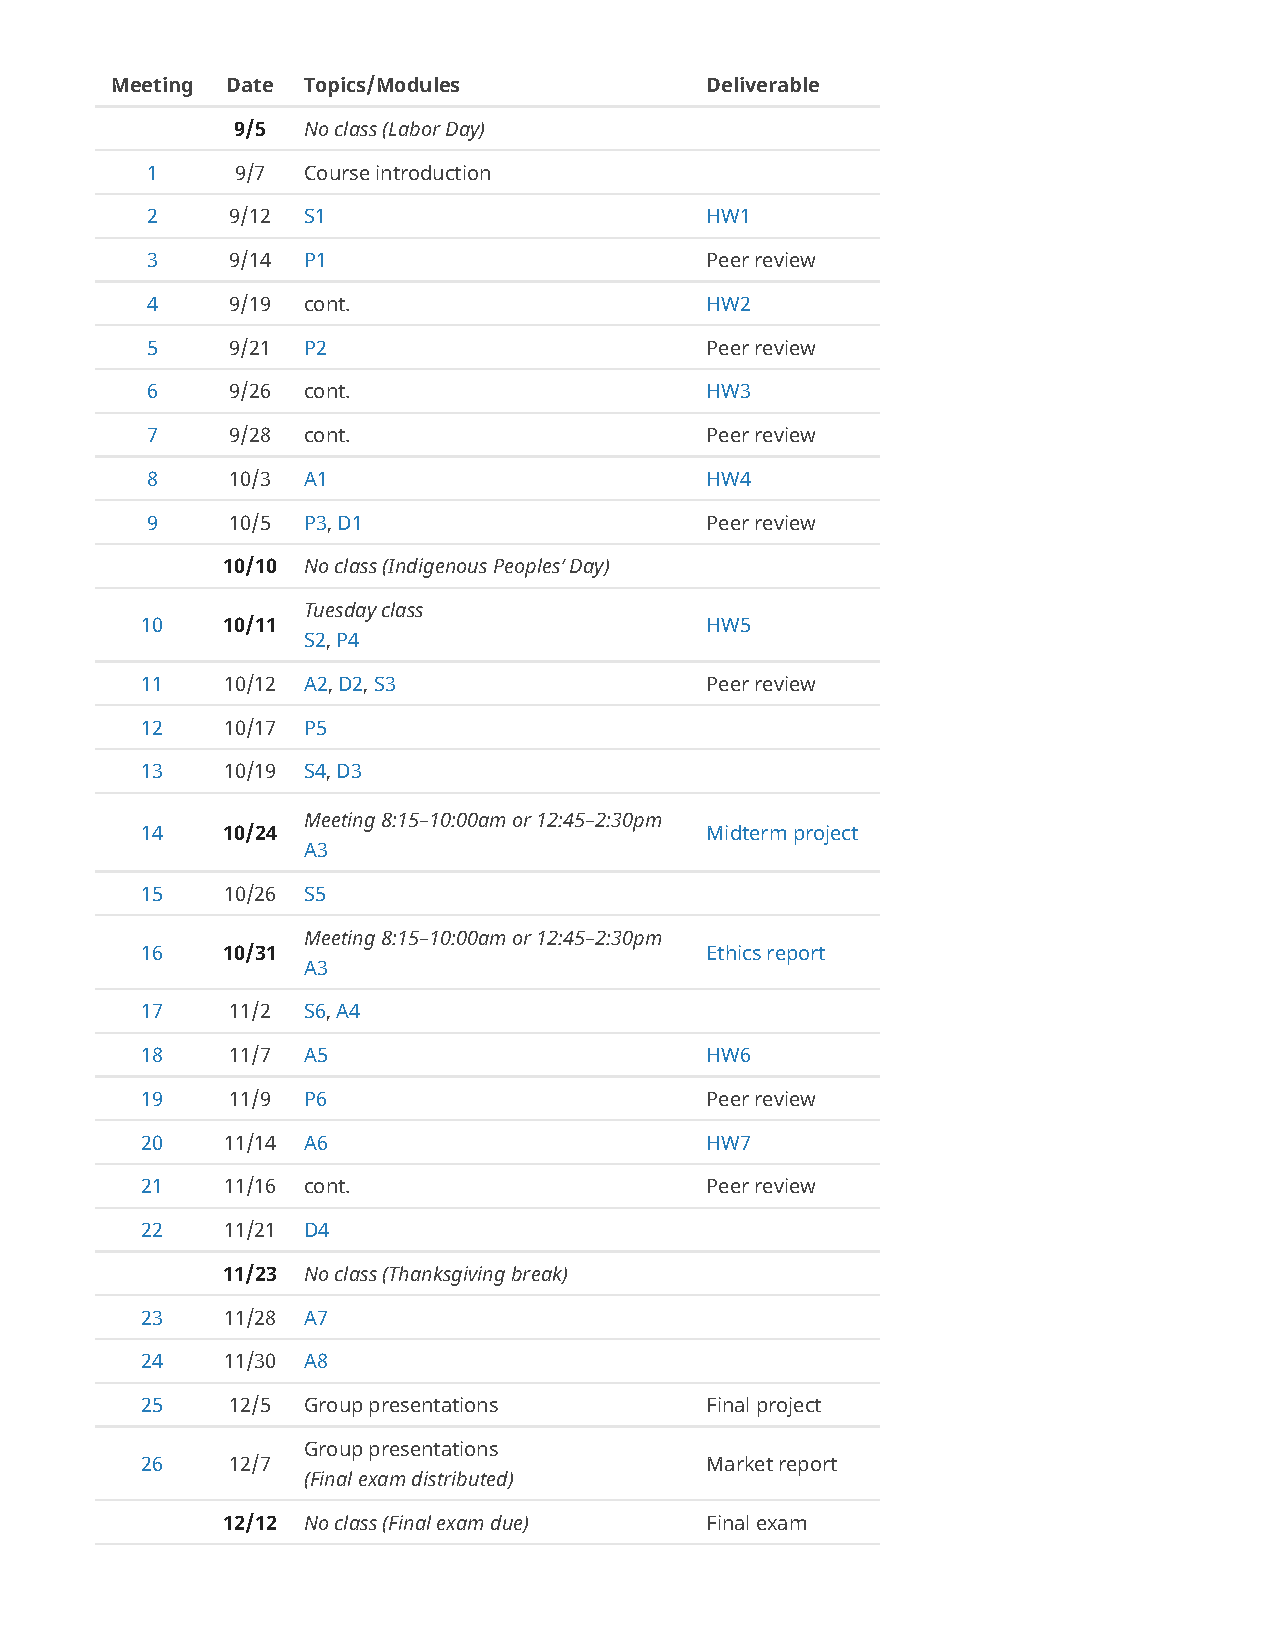
\includepdf[pages=-]{fin6200schedule}
\end{document}
